De acuerdo con Atienza \cite{Atienza2018}, Una vez que se completa el entrenamiento del modelo, la red predice los vectores que contienen los \textit{bounding boxes} y clases correspondientes. En algunos casos, dos o más bounding boxes se refieren al mismo objeto creando predicciones redundantes, por lo que para removerlas se utiliza el algoritmo de \textit{NMS} (\textit{Non maximum suppression}), el cual requiere conocer el vector de predicciones, con sus respectivos grados de confianza por clase y asignar un valor umbral el cual se denota $N_{t}$, cubriendo los requisitos ya mencionados el algoritmo define dos listas vacías $D$ y $S$ la primera almacenara los \textit{bounding boxes} finales y la segunda $S$ sus respectivos grados de confianza, Se asignan los bounding boxes iniciales y sus correspondientes grados de confianza a $B$ y $P$.
\\
\\
En las líneas 3 y 4 de la Figura \ref{NMS_algo} se selecciona el \textit{bounding box} con el grado de confianza más alto $p_{m}$ y es usado como referencia $b_{m}$. El \textit{bounding box} de referencia es agregado a la lista final de \textit{bounding boxes} $D$ y removido de la lista $B$, como se puede ver en la línea 5 de la Figura \ref{NMS_algo}, su puntuación es agregada a la lista $S$ Y removida de $P$. Para los \textit{bounding boxes} restantes si su IoU con su $b_{m}$ es mayor o igual al umbral $N_{t}$ estos serán borrados de $B$ y su correspondiente puntuación eliminada de $P$. Los pasos de las líneas 6, 9-11 de la Figura \ref{NMS_algo}, representan como son removidos los \textit{bounding boxes} con puntuaciones o grados de confianza pequeños. Después de que todos los \textit{bounding boxes} restantes hayan sido
examinados, se repite el proceso que comienza en la línea 3. El proceso continúa hasta
que la lista de cuadros delimitadores $B$ se ha vaciado. 
\\
\\
Por último en las líneas 7 y 8 se presenta la función de filtrado en caso de que se use la versión \textit{soft NMS}.
\begin{figure}[H]
    \centering
    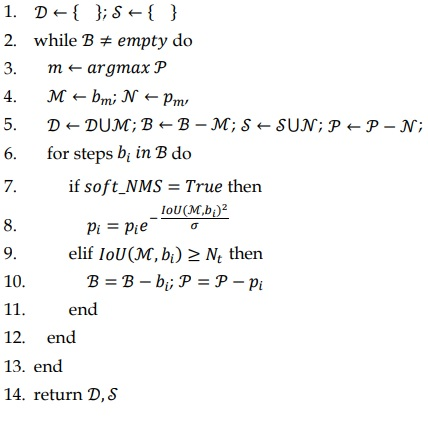
\includegraphics{Recursos/nms_algo.jpg}
    \caption[Algoritmo de NMS]{Algoritmo de NMS. {\footnotesize Fuente: \textit{Advanced Deep Learning with Keras} \cite[p.~376]{Atienza2018}}}
    \label{NMS_algo}
\end{figure}